\documentclass{article}
\usepackage{graphicx}
\usepackage{amsmath}
\usepackage{amsfonts}
\usepackage{amssymb}
\title{Metropolis-Hastings-Algorithm}
\date{January 2024}

\begin{document}

\maketitle
\section{Metropolis-Hastings (MH) algorithm}
Let $q(j \mid i)=Q_{i, j}$ be a proposal probability distribution with transition probability $Q$ satisfying
$$
q(j \mid i)>0 \Leftrightarrow q(i \mid j)>0 .
$$

Let $X_t=i$. The next state $X_{t+1}$ is realised in the following way.
1. Draw $j \sim q(\cdot \mid i)$ and $u \sim U[0,1]$.
2. If $u \leq \alpha(j \mid i)$ where
$$
\alpha(j \mid i)=\min \left\{1, \frac{p_j q(i \mid j)}{p_i q(j \mid i)}\right\}
$$
then set $X_{t+1}=j$, otherwise set $X_{t+1}=i$.
We initialise this with some $X_0=i_0$ satisfying $p_{i_0}>0$ and iterate for $t=1,2,3, \ldots T$ to simulate the samples we need. 
\newline
\textbf{Notation}
\begin{itemize}
    \item \( p_i \) is the probability of the system being in state \( i \) according to the target distribution, which is the distribution we're attempting to sample from using the Metropolis-Hastings algorithm.
    \item \( p_j \) is the probability of the system being in state \( j \) according to the same target distribution.
    \item  \( \frac{p_j}{p_i} \) reflects how much more likely we are to be in state \( j \) than in state \( i \) under the target distribution. If this ratio is greater than 1, it means state \( j \) is more likely than state \( i \); if it's less than 1, then state \( i \) is more likely than state \( j \).
\end{itemize}
\newline
\begin{itemize}
    \item \( q(j|i) \) is the probability of proposing state \( j \) as the next state given that the current state is \( i \). It's a part of the proposal distribution that suggests the next move.
    \item \( q(i|j) \) is the probability of proposing state \( i \) as the next state given that the current state is \( j \).
    \item  \( \frac{q(j|i)}{q(i|j)} \) is used in the acceptance probability to correct for any asymmetry in the proposal distribution. If the proposal distribution is symmetric, meaning \( q(j|i) = q(i|j) \), then this ratio is 1 and cancels out in the acceptance probability calculation. If it's not symmetric, this ratio ensures that the algorithm still satisfies detailed balance and therefore converges to the correct target distribution.
\end{itemize}
\newline
\subsection{Intuitive Explanation}
The Metropolis-Hastings algorithm can draw samples from any probability distribution with probability density $P(x)$, provided that we know a function $f(x)$ proportional to the density $P$ and the values of $f(x)$ can be calculated. The requirement that $f(x)$ must only be proportional to the density, rather than exactly equal to it, makes the Metropolis-Hastings algorithm particularly useful, because calculating the necessary normalization factor is often extremely difficult in practice.

The Metropolis-Hastings algorithm generates a sequence of sample values in such a way that, as more and more sample values are produced, the distribution of values more closely approximates the desired distribution. These sample values are produced iteratively, with the distribution of the next sample being dependent only on the current sample value, thus making the sequence of samples into a Markov chain. Specifically, at each iteration, the algorithm picks a candidate for the next sample value based on the current sample value. Then, with some probability, the candidate is either accepted, in which case the candidate value is used in the next iteration, or it is rejected in which case the candidate value is discarded, and current value is reused in the next iteration. The probability of acceptance is determined by comparing the values of the function $f(x)$ of the current and candidate sample values with respect to the desired distribution.
The Metropolis-Hastings (MH) algorithm is like playing a game where you're trying to explore different rooms in a mansion, and each room has a certain 'popularity' score. You want to spend time in each room proportionally to its popularity, but you don't know the popularity scores in advance.

Here's how the game works:
\begin{enumerate}
    \item Starting Point: You begin in one room (initial state \( X_0 \)).
    \item Propose a Move: You roll a die (draw \( j \)) to decide which room to explore next. This die is a bit quirky; depending on the room you're currently in, it's biased either for or against certain rooms (this bias is the proposal probability \( q(j \mid i) \)).
    \item  Random Chance: You flip a coin (draw \( u \) from a uniform distribution \( U[0,1] \)) to add some randomness to your decision.
    \item Make a Decision: Whether you move to the new room or stay in the current one depends on a comparison between the popularity of the current room and the proposed room, adjusted by the biases of the die. If the new room is popular enough compared to your current one (or the coin flip is particularly favorable), you move there; otherwise, you stay put.
\end{enumerate}

This game ensures that over time, you'll visit each room proportionally to its popularity, even though you're making your decisions with a biased die and a coin flip.
\newline
\subsection{Mathematical Explanation}
\newline
Mathematically, the Metropolis-Hastings algorithm simulates a Markov chain with the aim of generating samples from a probability distribution \( p \) that might be difficult to sample from directly.

Here's the step-by-step process:
\begin{enumerate}
    \item Current State: Let the current state be \( X_t = i \).
    \item Propose a New State: Draw a candidate new state \( j \) from a proposal distribution \( q(j \mid i) \).
    \item Random Uniform Draw: Generate a random number \( u \) from a uniform distribution \( U[0,1] \).
\item Acceptance Probability: Calculate the acceptance probability \( \alpha(j \mid i) \), which is the minimum between 1 and the\textit{ ratio of the target probabilities of the new and current states,} multiplied by the ratio of the proposal probabilities for the reverse and forward moves.
\item Accept or Reject: If \( u \) is less than or equal to \( \alpha(j \mid i) \), accept the move and set \( X_{t+1} = j \); otherwise, stay in the current state and set \( X_{t+1} = i \).
\end{enumerate}

This process is repeated for a large number of iterations \( T \), and after some initial 'burn-in' period, the states \( X_t \) can be considered as samples from the desired distribution \( p \). The condition \( q(j \mid i) > 0 \Leftrightarrow q(i \mid j) > 0 \) ensures that every state can potentially be visited, and the chain is not trapped in any subset of the state space.
\newline
\subsection{Comparison Rejection Sampling and MH Algo}
\newline
Compared with an algorithm like adaptive rejection sampling that directly generates independent samples from a distribution, MetropolisHastings and other MCMC algorithms have a number of \textit{disadvantages}:
\begin{itemize}
    \item The samples are autocorrelated. Even though over the long term they do correctly follow $P(x)$, a set of nearby samples will be correlated with each other and not correctly reflect the distribution. This means that effective sample sizes can be significantly lower than the number of samples actually taken, leading to large errors.
    \item Although the Markov chain eventually converges to the desired distribution, the initial samples may follow a very different distribution, especially if the starting point is in a region of low density. As a result, a burn-in period is typically necessary, where an initial number of samples are thrown away.

\end{itemize}
The samples are autocorrelated. Even though over the long term they do correctly follow $P(x)$, a set of nearby samples will be correlated with each other and not correctly reflect the distribution. This means that effective sample sizes can be significantly lower than the number of samples actually taken, leading to large errors.

\textit{Advantages:}
On the other hand, most simple rejection sampling methods suffer from the "curse of dimensionality", where the probability of rejection increases exponentially as a function of the number of dimensions. Metropolis-Hastings, along with other MCMC methods, do not have this problem to such a degree, and thus are often the only solutions available when the number of dimensions of the distribution to be sampled is high. As a result, MCMC methods are often the methods of choice for producing samples from hierarchical Bayesian models and other high-dimensional statistical models used nowadays in many disciplines.

\begin{figure}
    \centering
    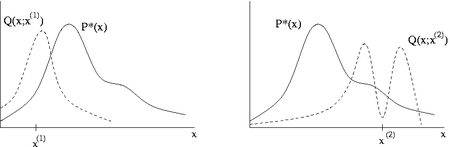
\includegraphics[width=1\linewidth]{ox-hilary/bayes-methods/figures/450px-Metropolis_hastings_algorithm.png}
\end{figure}
\begin{figure}
    \centering
    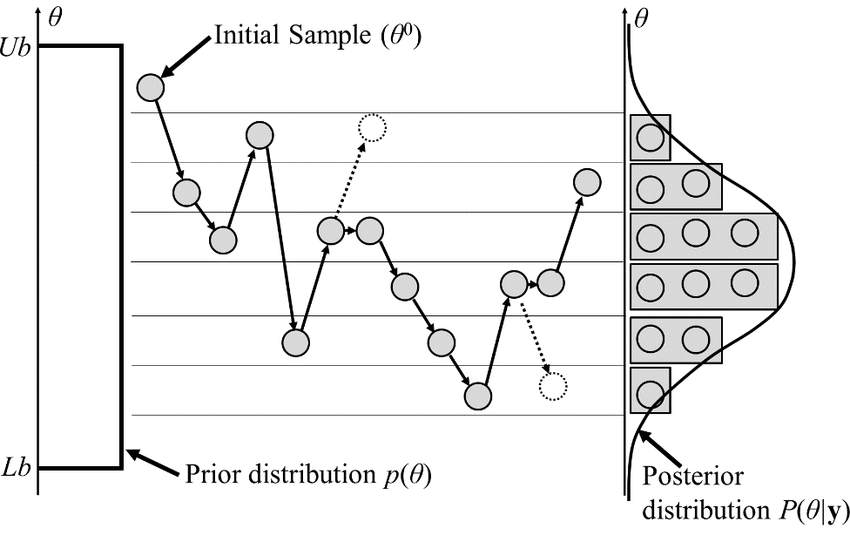
\includegraphics[width=0.5\linewidth]{ox-hilary/bayes-methods/figures/flow.png}
\end{figure}
\subsubsection{Continuous Case}

The candidate state $\theta^{\prime} \sim q\left(\theta^{\prime} \mid \theta\right)$ has distribution $q\left(d \theta^{\prime} \mid \theta\right)$. MCMC targeting $\pi(\theta), \theta \in \Omega$ : Let $X_t=\theta$.
\begin{enumerate}
    \item Draw $\theta^{\prime} \sim q(\cdot \mid \theta)$ and $u \sim U[0,1]$.
    \item  If $u \leq \alpha\left(\theta^{\prime} \mid \theta\right)$ where
\end{enumerate}
 
$$
\alpha\left(\theta^{\prime} \mid \theta\right)=\min \left\{1, \frac{\pi\left(\theta^{\prime}\right) q\left(\theta \mid \theta^{\prime}\right)}{\pi(\theta) q\left(\theta^{\prime} \mid \theta\right)}\right\}
$$
then set $X_{t+1}=\theta^{\prime}$, otherwise set $X_{t+1}=\theta$.

The rejection probability when the current state is $X_t=\theta$ is
$$
c(\theta)=1-\int_{\Omega} \alpha\left(\theta^{\prime} \mid \theta\right) q\left(d \theta^{\prime} \mid \theta\right)
$$
The transition distribution $ K(\theta, A)=\mathbb{P}\left(X_{t+1} \in A \mid X_t=\theta\right) $ is
$$
K\left(\theta, d \theta^{\prime}\right)=\alpha\left(\theta^{\prime} \mid \theta\right) q\left(d \theta^{\prime} \mid \theta\right)+c(\theta) \delta_\theta\left(d \theta^{\prime}\right) .
$$

The delta function $\delta_\theta\left(d \theta^{\prime}\right)$ satisfies $\int_A \delta_\theta\left(d \theta^{\prime}\right)=\mathbb{I}_{\theta \in A}$.
When $\theta^{\prime} \neq \theta$ the transition distribution has a simple unnormalised density
$$
K\left(\theta, \theta^{\prime}\right)=\alpha\left(\theta^{\prime} \mid \theta\right) q\left(\theta^{\prime} \mid \theta\right)
$$

\textbf{Detailed balance} 
$$
K\left(\theta, \theta^{\prime}\right) \pi(\theta)=K\left(\theta^{\prime}, \theta\right) \pi\left(\theta^{\prime}\right)
$$

\begin{itemize}
    \item Continuous Case Notation: We are now considering a continuous probability space. In this context, \(\Omega\) represents the space of all possible states, and \(\theta\) represents a random variable with a continuous probability density function (pdf) \( p(\theta) \). The pdf assigns probabilities to different continuous regions of \(\Omega\).
    \item  \( q(\theta'|\theta) \) := Proposal density is a function that generates a new candidate state \(\theta'\) given the current state \(\theta\), and \( \alpha(\theta'|\theta) \) is the acceptance probability, which determines whether to accept or reject the new state. The acceptance probability is calculated using the pdf of the current and proposed states, as well as the proposal density in both directions (from \(\theta\) to \(\theta'\) and vice versa). The minimum function ensures that this probability does not exceed 1.
    \item  \( c(\theta) \):= Rejection probability, represents the probability of rejecting a proposed new state. It is calculated by integrating the acceptance probability over the entire space \(\Omega\), subtracting it from 1.
    \item Transition Kernel: Finally, the transition probability \( P_{ij} \), which in the discrete case represents the probability of moving from state \( i \) to state \( j \), becomes a transition kernel \( K(\theta',\theta) \) in the continuous case. This kernel is a conditional probability distribution and it indicates the probability that the chain moves into a set \( A \) in the next step, given the current state \( \theta \).
\end{itemize}

\begin{figure}
    \centering
    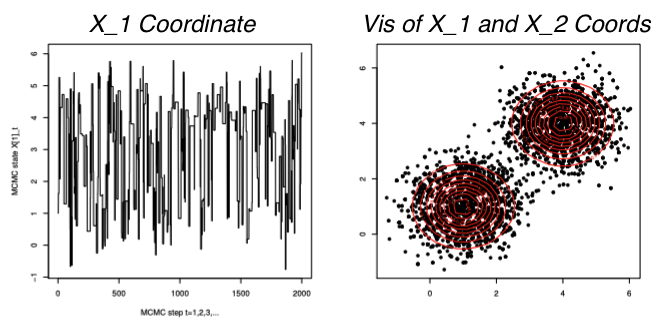
\includegraphics[width=1\linewidth]{ox-hilary/bayes-methods/figures/Screenshot 2024-01-24 at 22.54.48.png}
    \caption{MCMC targeting a mixture of bivariate normals: (Left) MCMC trace of θ(t)  1 plotted  against t for t = 1, ..., 2000; (Right) scatter plot of sampled parameter vectors (θ(t)  1 , θ(t)  2 ), t =  1, ..., 2000. 
}
\end{figure}

\end{document}